%!TEX root = ./main.tex

\begin{figure}[!t]
    \centering
    \vspace{-4pt}
    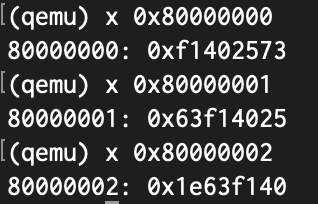
\includegraphics[scale=0.75]{figures/qemu.png}
    \vspace{-5pt}
    \caption {
        Debugging Memory Addresses with QEMU
    }
    \label{debug-memory-address-qemu}
\end{figure}

\section{Tool}

As shown in \ref{debug-memory-address-qemu}, debugging a range of memory addresses in QEMU is not easy.
%
\tool aims to fix this by providing two key features.
%
The first feature is the memory address viewer, which will allow developers to see memory in real time.
%
QEMU is currently set up to allow developers to see a memory address, but they must type the memory address they want to see.
%


\subsection{Part 1}

\subsection{Part 2}